%% The following is a directive for TeXShop to indicate the main file
%%!TEX root = diss.tex

\chapter{Methods}
\label{ch:Methods}

\section{Initial Simulation}
\label{sec:experiment}
For my thesis project, I intend to create a fast simulation of charged particles travelling through the aerogel in the proposed \ac{EMPHATIC} \ac{ARICH} detector, and determine the distribution of resultant photons that strike the detector. 

These simulations will be created using \textsc{root}: a scientific computing framework based off C++ and developed at CERN \cite{root}. Our simulation will take in as input the velocity and $\theta$ and $\phi$ angles of the particle with respect to the axis of the beam. Using \textsc{root}, a vast number of particles may be simulated, whose velocities and trajectories are based off these inputs, but randomly distributed according to the resolution of the upstream particle trackers. The photons emitted by the particles travelling through the aerogel have a fixed angle $\theta$ with respect to the momentum of the particle, determined by Equation \ref{eq:cherenkovAngle}, but vary randomly with respect to their $\phi$ angle. The average number of photons emitted by each of these particles is determined by Equation \ref{eq:photonNumber}. These photons will then travel out of the aerogel and have some chance of striking the detector. The detector itself has some probability of detecting the hit, based off its efficiency. 

Once a simulation has been created to handle this procedure, it will be verified against an already-existing simulation of the full detector configuration. The full simulation is handled with \textsc{Geant4}, a C++ based software toolkit designed for Monte Carlo simulations of particles travelling through complex detector geometry  \cite{geant4}.

Once this simple simulation has been verified, the effects of photon scattering in the aerogel will be incorporated into the simulation. The transmittance of these photons through the aerogel has contributions from scattering and absorption effects, but the dominant contribution is from Rayleigh scattering \cite{aerogelRefraction}. The probability that a photon  undergoes Rayleigh scattering is proportional to $\lambda^{-4}$, where $\lambda$ is the wavelength of the light, and the angular distribution of scattered photons is proportional to $1 + \cos^2(\theta)$ \cite{rayleigh}. The known optical transmittance of the aerogel \cite{aerogelRefraction} may be fit to obtain the probability that a photon will undergo Rayleigh scattering after travelling some distance. We enhance our simulation by adding this random scattering effect to each photon: we randomly select whether the photon will have scattered at each point in its trajectory based off this probability, and generate a new $\theta$ and $\phi$ for the photon. 

After simulating thousand of particles entering the \ac{ARICH} with a given velocity and trajectory, we can average over all the photons hitting the detector to get a probability distribution. An example of a probability distribution is shown in Figure \ref{fig:particleRings}. This probability distribution can then be used for particle identification.

\begin{figure}[h!]
\centering
\resizebox{0.8\textwidth}{!}{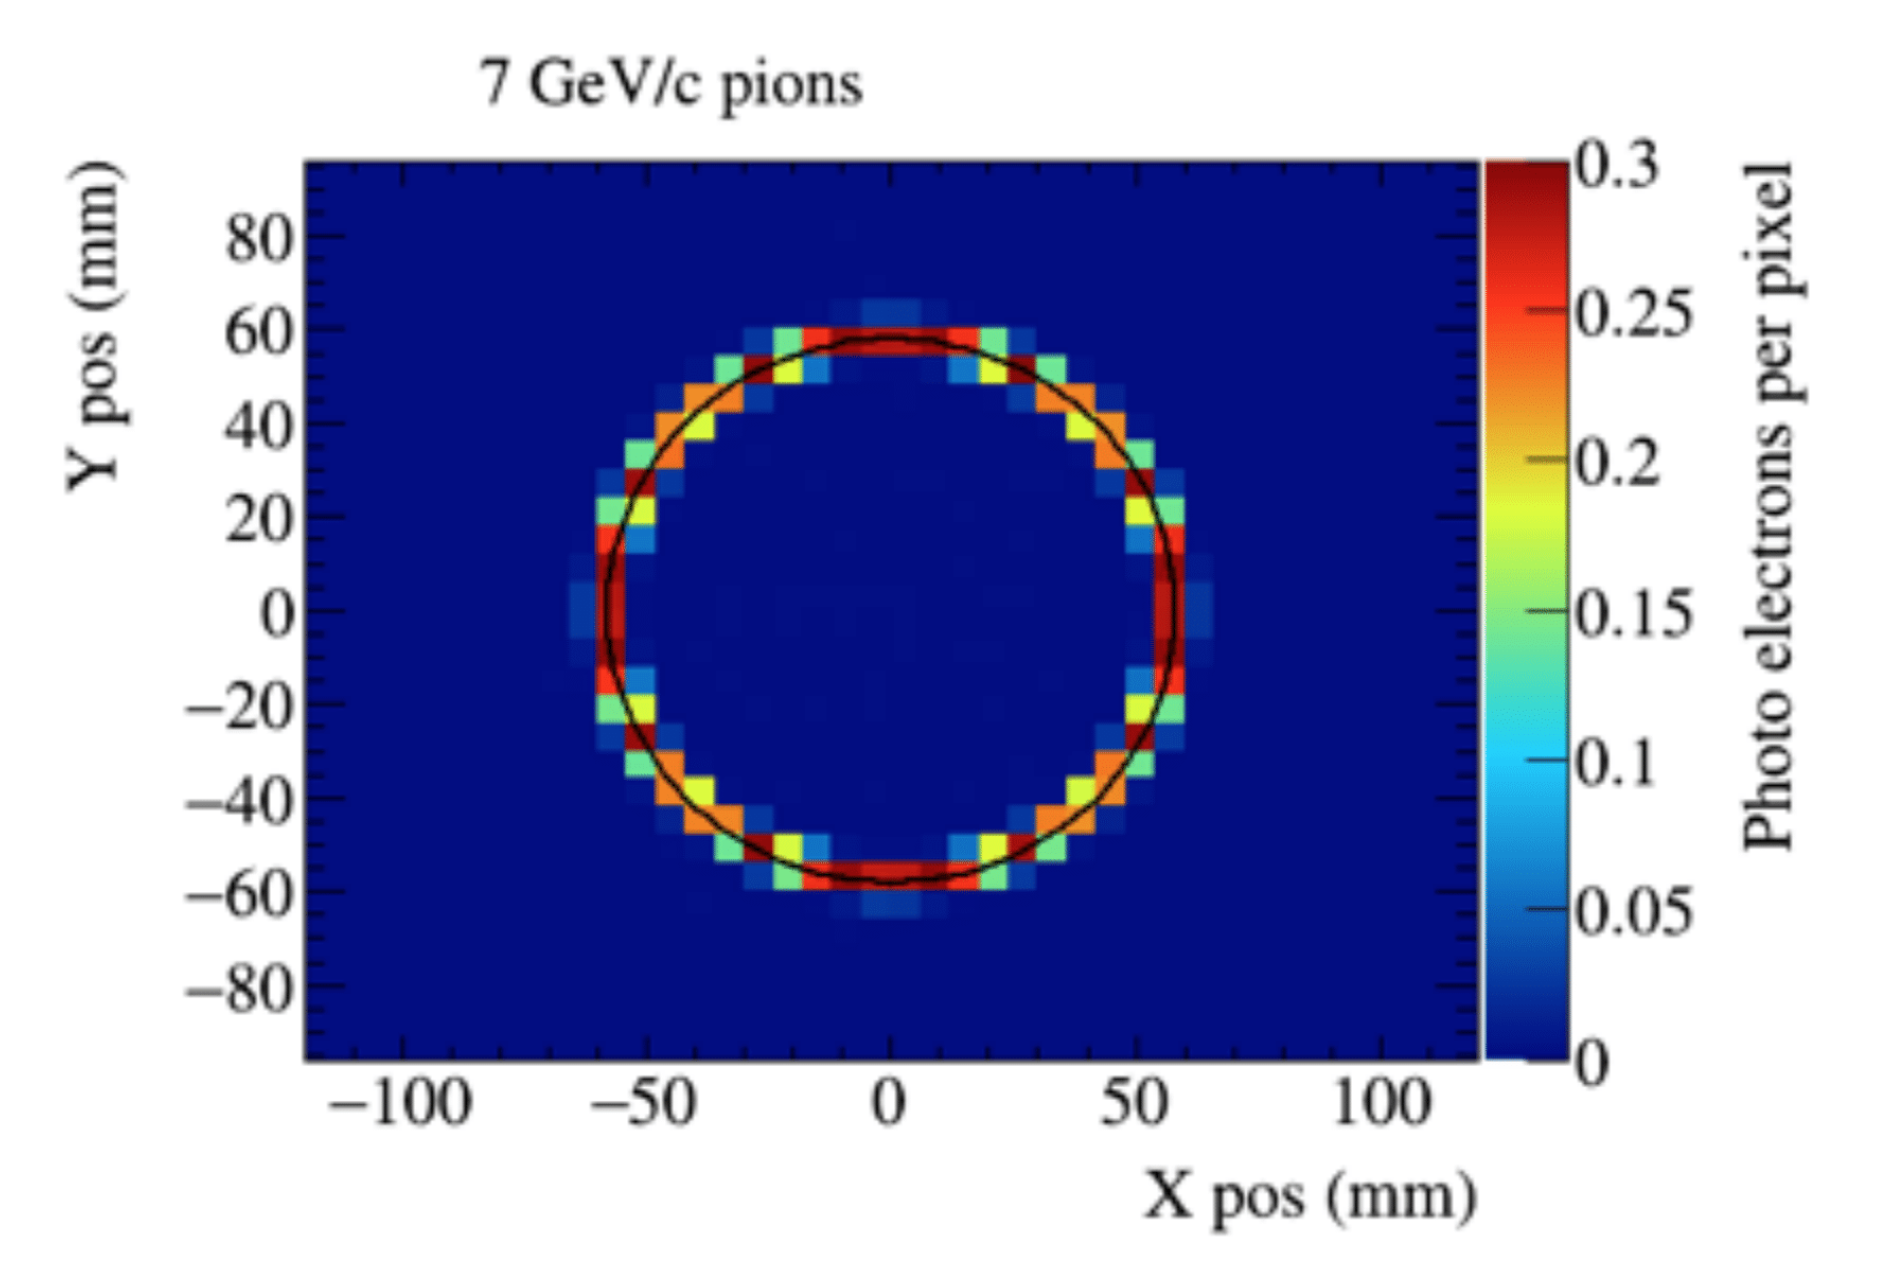
\includegraphics{./figs/particleRing.png}}
\caption[Example of a simulated photon probability distribution]{Example of the photon probability distribution on a detector plane resulting from a simulation of the photons emitted by 10,000 pions with a momentum of 7 GeV/c emitting Cherenkov radiation. The photons were simulated using \textsc{Geant4}. The figure was obtained with permission from the \textsc{EMPHATIC} group.}

\label{fig:particleRings}       % Give a unique label to the figure. 
\end{figure}

\section{Particle Identification}
\label{sec:particleIdentification}
In order to identify particles using the \ac{ARICH} detector, a particle likelihood method is used \cite{richImpact, belleArich}. For this method, we take the known momentum of the particle, and use Equation \ref{eq:relMass} to determine the expected velocity for different candidate particles masses. The candidate particles of interest to the experiment are protons, electrons, pions, and kaons. For each velocity hypothesis, we run 10,000 simulations of particles moving at that velocity, with the same measured initial trajectory as input. For each pixel of the detector, this procedure will give a value $\lambda_i(\beta)$, equal to the expected number of photons striking pixel $i$ in the detector due to a particle of velocity $\beta$. 

For a given particle event, we will detect $N_i$ photons in each pixel $i$. In reality, the PMTs are only capable of registering whether or not a photon has been detected - if multiple photons strike a single pixel in a very short amount of time, it will not be able to distinguish the number detected, so we just know if $N_i = 0$ or $N_i > 0$.

The probability that zero photons strike pixel $i$ is given by the Poisson distribution for zero events:
$$ P_i(N_i=0; \beta) = e^{-\lambda_i(\beta)} $$
 The probability that one or more photons strike pixel $i$ must then be:
$$ P_i(N_i>1; \beta) = 1 - e^{-\lambda_i(\beta)} $$

By multiplying the probabilities of getting the observed result in each pixel $i$ of the detector, we calculate the likelihood for that value of $\beta$:

$$L_\beta = \prod_{i}P_i(N_i; \beta)$$

For convenience, we actually compute:
\begin{equation}
    \label{eq:loglikelihood}
    -2\ln(L_\beta) = \sum_i \ln(P_i(N_i; \beta))
\end{equation}


We compute the log-likelihood of our data matching each of particle hypothesis, and choose that which minimizes the value.

\section{Modifying the simulation}
After having created the simulation, I will test its ability to adequately discriminate between different particles for a broad range of particle momenta and trajectories. Following these calculations, greater realism will be added to the simulation. The specific placement of PMTs in the photon detection array can be modelled to get a more accurate picture of the detector's angular resolution and efficiency. The effects of different detector configurations may be investigated in order to get the best possible particle discrimination. 

A possible change to the detector configuration is the addition mirrors along the space between the aerogel radiator and the photon detectors. This would allow photons emitted at high angles to reflect off the mirrors and back onto the detector, increasing the total angular coverage of the detector. The effects of this addition on the detector's particle discrimination ability can also be simulated.




\endinput

Any text after an \endinput is ignored.
You could put scraps here or things in progress.
